\documentclass[notes,blackandwhite,mathsans]{beamer}

\usepackage{amsmath}
\usepackage{amssymb}
\usepackage{graphicx}
\usepackage{fancybox}
\usepackage{booktabs}
\usepackage{multirow,pxfonts}
\usepackage{cmbright}
\usepackage{color}
\usepackage{xcolor}
\usepackage{enumitem}
\usepackage{animate}
\usepackage{changepage}

\usepackage[T1]{fontenc}
\fontencoding{T1}  
\usepackage[utf8]{inputenc}


\usefonttheme{default}
\setbeamercovered{invisible}
\beamertemplatenavigationsymbolsempty

\makeatletter
\setbeamertemplate{footline}
{
  \leavevmode
  \hbox{
  \begin{beamercolorbox}[wd=0.97\paperwidth,ht=2.25ex,dp=2ex,right]{}
{\color{mcxs3} \insertframenumber{} / \inserttotalframenumber}
  \end{beamercolorbox}}%
}



\definecolor{mcxs1}{HTML}{05386B}
\definecolor{mcxs2}{HTML}{379683}
\definecolor{mcxs3}{HTML}{5CDB95}
\definecolor{mcxs4}{HTML}{8EE4AF}
\definecolor{mcxs5}{HTML}{EDF5E1}
\setbeamercolor{frametitle}{fg=mcxs2}
\AtBeginDocument{\color{mcxs1}}

%\setbeamercolor{itemize text}{fg=mcxs5}
\setbeamercolor{itemize item}{fg=mcxs1}
\setbeamercolor{itemize subitem}{fg=mcxs2}
\setbeamercolor{enumerate item}{fg=mcxs1}
\setbeamercolor{description item}{fg=mcxs1}

\setbeamertemplate{itemize item}[triangle]
\setbeamertemplate{itemize subitem}[circle]



\begin{document}
%\fontfamily{pag}\selectfont
%\setbeamerfont{title}{family=\fontfamily{pag}\selectfont}
%\setbeamerfont{frametitle}{family=\fontfamily{pag}\selectfont}
%\setbeamerfont{framesubtitle}{family=\fontfamily{pag}\selectfont}



\begin{frame}
\centering
\includegraphics[scale=1.87]{mcxs.png}
\end{frame}






{\setbeamercolor{background canvas}{bg=mcxs5}
\begin{frame}

\vspace{1cm}
\begin{tabular}{rl}
&\textbf{\LARGE\color{mcxs2} Macroeconometrics}\\[8ex]
\textbf{\Large Lecture 5}&\textbf{\Large\color{mcxs2}Understanding unit-rooters}\\[19ex]
&\textbf{Tomasz Wo\'zniak}\\[1ex]
&{\small\color{mcxs2} Department of Economics}\\
&{\small\color{mcxs2}University of Melbourne}
\end{tabular}

\end{frame}
}



{\setbeamercolor{background canvas}{bg=mcxs5}
\begin{frame}

\vspace{1cm} \textbf{\color{mcxs2}Concepts}

\bigskip\textbf{\color{mcxs2}Autoregressions}

\bigskip\textbf{\color{mcxs1}Random walk processes}

\bigskip\textbf{\color{mcxs1}Inference}

\bigskip\textbf{\color{mcxs1}A helicopter tour}


\small
\vspace{1cm} Useful readings: \\ \footnotesize
\smallskip{\color{mcxs2}Sims, Uhlig (1991) Understanding Unit Rooters: A Helicopter Tour, Econometrica}

\bigskip\normalsize Materials:\\[1ex] \footnotesize
{\color{mcxs2}An R file} \texttt{05 mcxs.R}, \texttt{06 mcxs.R} {\color{mcxs2}for the reproduction the results}\\
{\color{mcxs2}Shiny interactive apps:} \texttt{05shiny-ar1.R} {\color{mcxs2}and} \texttt{05shiny-ar2.R}

\end{frame}
}



%{\setbeamercolor{background canvas}{bg=mcxs5}
%\begin{frame}
%
%\bigskip\textbf{\color{mcxs1}Objectives.}
%\begin{itemize}[label=$\blacktriangleright$]
%\item {\color{mcxs1}To introduce autocorrelations as a measure of persistence of time series}
%\item {\color{mcxs1}To analyse autocorrelation patterns of stochastic processes}
%\item {\color{mcxs1}To understand models by the dynamic patterns of data they can capture}
%\end{itemize}
%
%\bigskip\textbf{\color{mcxs2}Learning outcomes.}
%\begin{itemize}[label=$\blacktriangleright$]
%\item {\color{mcxs2}Interpreting autocorrelograms of data}
%\item {\color{mcxs2}Deriving autocorrelation pattern of a model}
%\item {\color{mcxs2}Analysing random walk processes}
%\end{itemize}
%
%\end{frame}
%}











{\setbeamercolor{background canvas}{bg=mcxs5}
\begin{frame}

\begin{adjustwidth}{-0.5cm}{0cm}
%\FlushLeft
\vspace{8.3cm}\Large
\textbf{{\color{mcxs1}Concepts} {\color{white}}}
\end{adjustwidth}

\end{frame}
}




\begin{frame}{Strict stationarity}

\vspace{0.3cm}
{\color{mcxs2}A time series }${y_t}$ {\color{mcxs2}is said to be} {\color{mcxs2}strictly stationary} {\color{mcxs2}if the joint distribution of} $(y_{t_1}, \dots , y_{t_k})$ {\color{mcxs2}is identical to that of} $(y_{t_1+s}, \dots , y_{t_k+s})$ {\color{mcxs2}for all $t$, where $k$ is an arbitrary positive integer and} $(t_1, \dots , t_k)$ {\color{mcxs2}is a collection of $k$ positive integers:}
$$ p(y_{t_1}, \dots , y_{t_k}) = p(y_{t_1+s}, \dots , y_{t_k+s}). $$

\end{frame}


\begin{frame}{Covariance stationarity}


\vspace{0.3cm}
{\color{mcxs2}A time series} ${y_t}$ {\color{mcxs2}is said to be} {\color{mcxs2}covariance or weakly stationary} {\color{mcxs2}if both the} mean {\color{mcxs2}of} $y_t$ {\color{mcxs2}and the} covariance {\color{mcxs2}between} $y_t$ and $y_{t-s}$ {\color{mcxs2}are} {\color{mcxs2}time invariant}, {\color{mcxs2}where} $s$ {\color{mcxs2}is an arbitrary integer:}
\begin{align*}
\mathbb{E}[y_t] &= \mu, \\
\mathbb{C}\text{ov}[y_t, y_{t-s}] &= \gamma_s,
\end{align*}
{\color{mcxs2}where:}\\
\hspace{0.3cm}$\gamma_0 = \mathbb{V}\text{ar}[y_t]$\\
\hspace{0.3cm}$ \gamma_{-s} = \gamma_s $

\end{frame}




\begin{frame}{Unconditional moments}


\textbf{Expected value:}
$$ \mathbb{E}[y_{t}] = \int_{\mathbb{R}}y_tp(y_t)dy_t $$


\textbf{Covariance matrix.}
$$ \mathbb{V}\text{ar}[y_{t}] = \mathbb{E}\left[\left(y_{t} - \mathbb{E}[y_{t}]\right)\left(y_{t} - \mathbb{E}[y_{t}]\right)'\right] $$


\textbf{Autocovariance.}
$$ \mathbb{C}\text{ov}[y_{t}, y_{t-s}] = \mathbb{E}\left[\left(y_{t} - \mathbb{E}[y_{t}]\right)\left(y_{t-s} - \mathbb{E}[y_{t-s}]\right)'\right] $$

\end{frame}





\begin{frame}{Sample moments}

\textbf{Sample mean.}
$$ \bar{y} = \frac{1}{T}\sum_{t=1}^{T}y_t $$


\textbf{Sample covariance matrix.}\\
$$ \hat{\gamma}_0 = \frac{1}{T}\sum_{t=1}^{T}\left[(y_{t} - \bar{y})(y_{t} - \bar{y})'\right] $$


\textbf{Sample autocovariance.}
$$ \hat{\gamma}_s = \frac{1}{T-s}\sum_{t=s+1}^{T}\left[(y_{t} - \bar{y})(y_{t-s} - \bar{y})'\right] $$

\end{frame}


\begin{frame}{Autocorrelation }


\textbf{Autocorrelation function - ACF.}
$$ \rho_s = \mathbb{C}\text{orr}[y_{n.t}, y_{n.t-s}] = \frac{\mathbb{E}\left[\left(y_{n.t} - \mathbb{E}[y_{n.t}]\right)\left(y_{n.t-s} - \mathbb{E}[y_{n.t-s}]\right)\right]}{\sqrt{ \mathbb{V}\text{ar}[y_{n.t}] \mathbb{V}\text{ar}[y_{n.t-s}] } }  $$

\bigskip\textbf{Sample autocorrelation.}
$$ \hat{\rho}_s = \frac{\sum_{t=s+1}^{T}[(y_{n.t} - \bar{y}_n)(y_{n.t-s} - \bar{y}_n)]}{\sqrt{\left[\sum_{t=s+1}^{T}(y_{n.t} - \bar{y}_n)^2 \right]\left[\sum_{t=1}^{T-s}(y_{n.t-s} - \bar{y}_{n.s})^2 \right]}} $$


\bigskip{\color{mcxs2}Assume covariance stationarity:}
$$\rho_s = \rho_{-s} = \frac{\gamma_s}{\gamma_0} $$


\end{frame}




\begin{frame}{White noise process}

{\color{mcxs2}A stochastic process} $\epsilon_t$ {\color{mcxs2}is called a} {\color{mcxs2}white noise} {\color{mcxs2}if} $\{\epsilon_t\}$ {\color{mcxs2}is an i.i.d. sequence:}
\begin{align*}
\mathbb{E}[\epsilon_t] &= 0 \\
\mathbb{V}\text{ar}[\epsilon_t] &= \sigma_{\epsilon}^2  < \infty \\
\mathbb{C}\text{ov}[\epsilon_t, \epsilon_{t-s}] &= 0 \qquad \forall s\neq0
\end{align*}

{\color{mcxs2}Denoted by}
$$ \epsilon_t \sim iid\left(0,\sigma_{\epsilon}^2 \right) $$

\bigskip\textbf{Gaussian white noise process.}
$$ \epsilon_t \sim iid\mathcal{N}\left(0,\sigma_{\epsilon}^2 \right) $$

\end{frame}








{\setbeamercolor{background canvas}{bg=mcxs5}
\begin{frame}

\begin{adjustwidth}{-0.5cm}{0cm}
%\FlushLeft
\vspace{8.3cm}\Large
\textbf{{\color{mcxs2}Autoregressions} {\color{white}}}
\end{adjustwidth}

\end{frame}
}



\begin{frame}{Autoregressions}

\textbf{AR($p$) model.}
\begin{align*}
y_t &= \mu_0 + \alpha_1y_{t-1} + \dots + \alpha_p y_{t-p} + \epsilon_t  \\
\epsilon_t&|y_{t-1},\dots, y_{t-p} \sim iid(0,\sigma_{\epsilon}^2)
\end{align*}

\bigskip\textbf{Exogeneity assumption in time series.}
$$ \mathbb{E}[\epsilon_t|y_{t-1},\dots, y_{t-p}] = 0 $$


\end{frame}


\begin{frame}{Autoregressions}

\textbf{AR($p$) model: alternative notations.}
\begin{align*}
y_t &= \mu_0 + \alpha_1y_{t-1} + \dots + \alpha_p y_{t-p} + \epsilon_t  \\
y_t - \alpha_1y_{t-1} - \dots - \alpha_p y_{t-p} &= \mu_0  + \epsilon_t  \\
\left( 1- \alpha_1L - \dots -\alpha_pL^p \right)y_t &= \mu_0 + \epsilon_t\\
\alpha(L) y_t &= \mu_0 + \epsilon_t
\end{align*}
$L$ {\color{mcxs2}denotes the lag operator such that} $L^sy_t=y_{t-s}$ {\color{mcxs2}and} $L^sc=c$

\bigskip\textbf{AR($p$) model: matrix notation.}
$$Y = X \beta + E  $$\footnotesize
$$ \underset{\color{mcxs2}(p+1\times1)}{\beta} = \begin{bmatrix} \mu_0\\ \alpha_1\\ \vdots \\ \alpha_p \end{bmatrix} \quad \underset{\color{mcxs2}(T\times1)}{Y} = \begin{bmatrix} y_1\\ \vdots \\ y_T \end{bmatrix} \quad \underset{\color{mcxs2}(p+1\times1)}{x_t'} = \begin{bmatrix} 1\\ y_{t-1}\\ \vdots \\ y_{t-p} \end{bmatrix} \quad \underset{\color{mcxs2}(T\times p+1)}{X} = \begin{bmatrix} x_1\\ \vdots \\ x_T \end{bmatrix}\quad \underset{\color{mcxs2}(T\times1)}{E} = \begin{bmatrix} \epsilon_1\\ \vdots \\ \epsilon_T \end{bmatrix}$$

\end{frame}





%\begin{frame}{Exercise!}
%
%\textbf{AR(p) model in matrix notation.}
%\begin{align*} 
%Y &= X\beta + E\\
%E|X &\sim\mathcal{N}\left(\mathbf{0}_T, \sigma^2I_T\right)
%\end{align*} 
%
%\textbf{Likelihood function.}
%\begin{equation*}
%L\left(\beta,\sigma^2|Y,X\right) \propto\left( \sigma^2 \right)^{-\frac{T}{2}}\exp\left\{ -\frac{1}{2}\frac{1}{\sigma^2}(Y- X\beta)'(Y- X\beta) \right\}
%\end{equation*}
%
%\textbf{Prior distribution.}
%$$ p\left(\sigma^2\right)=\mathcal{IG}2(\underline{s},\underline{\nu})\propto \left(\sigma^2\right)^{-\frac{\underline{\nu}+2}{2}}\exp\left\{ -\frac{1}{2}\frac{\underline{s}}{\sigma^2} \right\} $$
%
%\bigskip\Large
%{\color{mcxs2}\textbf{The task:} derive} $p\left(\sigma^2|Y,X,\beta\right)$
%
%\end{frame}





\begin{frame}{Autoregressions: stationarity}


{\color{mcxs2}An} AR($p$) {\color{mcxs2}model is called {\color{mcxs2}stationary} if:}
$$ \alpha(z) = 0 \qquad\text{{\color{mcxs2} for complex numbers} $z$ {\color{mcxs2}with} } |z|>1,$$

{\color{mcxs2}that is:}
$$1 - \alpha_1 z - \dots - \alpha_p z^p = 0 \qquad\text{\color{mcxs2} for } |z|>1 \text{ \color{mcxs2} and }z\in\mathbb{C}.$$

\bigskip{\color{mcxs2}Modulus of a complex number} $z = a + ib$ {\color{mcxs2}is:}
$$ |z| = \sqrt{a^2 + b^2} $$

\end{frame}




{\setbeamercolor{background canvas}{bg=mcxs5}
\begin{frame}{Unit circle}

\centering
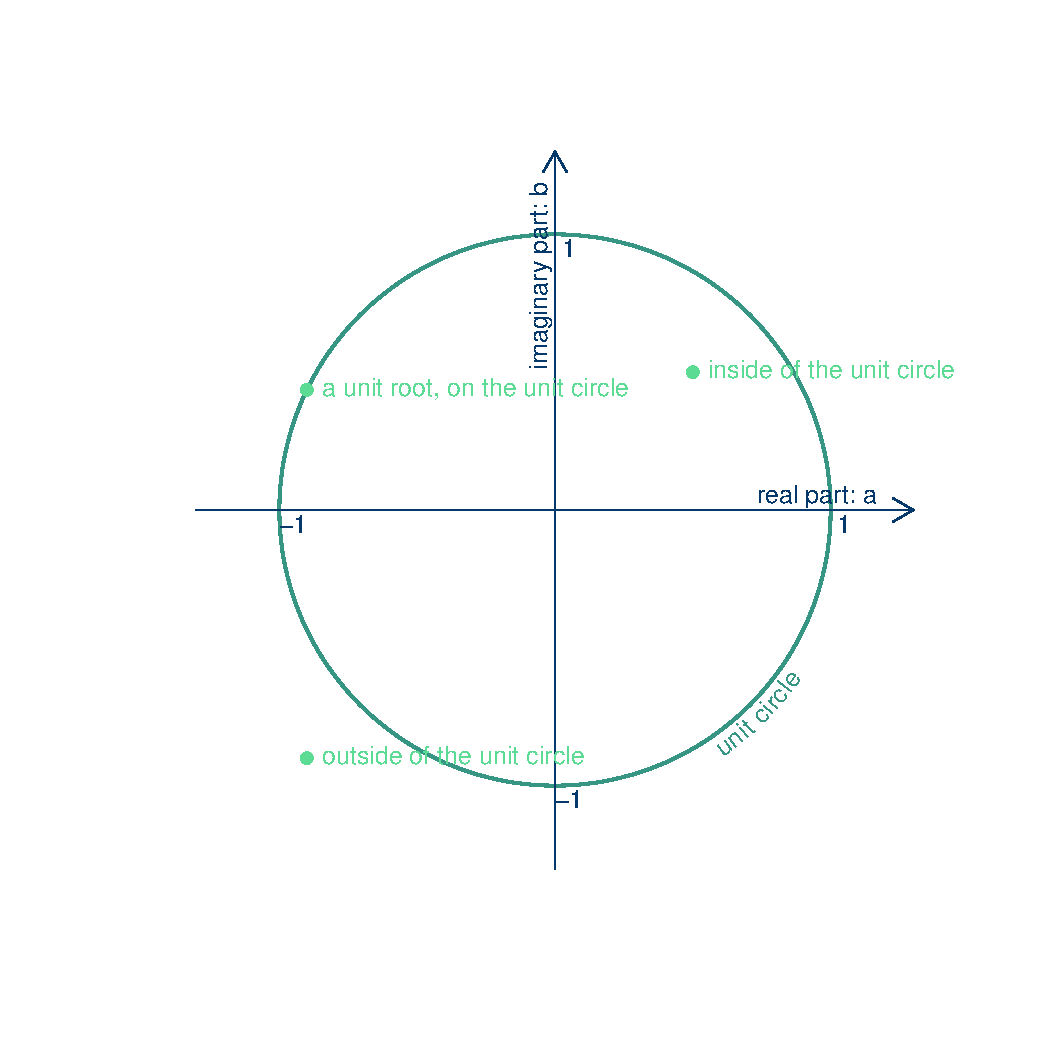
\includegraphics[scale=0.55, trim=0cm 3cm 0cm 2cm]{grphs/05unitcircle.pdf}

\bigskip{\color{mcxs2}The unit circle is given by equation:} $1^2 = a^2 + b^2$
\end{frame}
}




\begin{frame}{Autoregressions: invertibility}

{\color{mcxs2}A stationary} AR(${\color{mcxs1}p}$) {\color{mcxs2}model has an} MA(${\color{mcxs2}\infty}$) {\color{mcxs2}representation:}
\begin{align*}
\alpha(L)y_t &= \mu_0 + \epsilon_t \\
&\\
y_t &= \alpha(L)^{-1}\mu_0 + \alpha(L)^{-1}\epsilon_t \\
&= \mu + \phi(L)\epsilon_t\\
&= \mu + \epsilon_t + \phi_1 \epsilon_{t-1} + \phi_2\epsilon_{t-2} + \dots
\end{align*}

{\color{mcxs2}where:}
$$ \phi_j = \sum_{i=1}^{j}\phi_{j-i}\alpha_i, $$
{\color{mcxs2}for} $j=0,1,2, \dots$, {\color{mcxs2}and} $\phi_0 = 1$, {\color{mcxs2}and} $\alpha_i = 0$ {\color{mcxs2}for} $i>p$.
\end{frame}




\begin{frame}{Autoregressions: invertibility}

{\color{mcxs2}Consider a stationary} AR(1) {\color{mcxs2}model:}
\begin{align*}
y_t &= \mu_0 +\alpha_1 y_{t-1} + \epsilon_t \\
y_t -\alpha_1 y_{t-1} &= \mu_0 + \epsilon_t \\
(1-\alpha_1L)y_t &= \mu_0 + \epsilon_t 
\end{align*}


\vspace{0.5cm}{\color{mcxs2}It has an} MA($\infty$) {\color{mcxs2}representation:}
\begin{align*} 
y_t &= \frac{\mu_0}{1-\alpha_1} + \epsilon_t + \alpha_1 \epsilon_{t-1} + \alpha_1^2 \epsilon_{t-2} + \alpha_1^3 \epsilon_{t-3} + \dots\\
 &= \mu + \epsilon_t + \phi_1 \epsilon_{t-1} + \phi_2\epsilon_{t-2} + \dots
\end{align*}

\bigskip\textbf{Inverting polynomial of order 1:}
$$ (1 - az )^{-1} = 1 + \sum_{i=1}^{\infty} a^i z^i $$
\end{frame}






\begin{frame}{Autoregressions: unconditional moments }


\textbf{Unconditional mean.}\\
{\color{mcxs2}Assume stationarity.}
\begin{align*}
\mu = \mathbb{E}[y_t] &= \mathbb{E}[\alpha(1)^{-1}\mu_0 + \alpha(L)^{-1}\epsilon_t ] \\
&= \frac{\mu_0}{\alpha(1)} + \alpha(L)^{-1}\mathbb{E}[\epsilon_t] \\
&= \frac{\mu_0}{\alpha(1)} + \alpha(L)^{-1}\mathbb{E}\left[\mathbb{E}[\epsilon_t|y_{t-1},\dots,y_{t-p}]\right] \\[2ex]
\mu &= \frac{\mu_0}{1 - \alpha_1 - \dots - \alpha_p } \\
&\text{\color{mcxs2}given that: }\alpha_1 + \dots + \alpha_p \neq 1
\end{align*}

\textbf{The Law of Iterated Expectations.}\\
$$ \mathbb{E}\left[\epsilon_t\right] \overset{LIE}{=} \mathbb{E}\left[\mathbb{E}[\epsilon_t|y_{t-1},\dots,y_{t-p}]\right] \overset{exogeneity}{=} \mathbb{E}\left[0\right] = 0$$
\end{frame}


\begin{frame}{Autoregressions: autocorrelations}
\small

\textbf{AR(1) model.}
\begin{description}
\item[Step 1:] {\color{mcxs2}Use} $\mu_0 = \mu(1 - \alpha_1)${\color{mcxs2}, to write the model as:}
$$ y_t - \mu = \alpha_1(y_{t-1} - \mu) + \epsilon_t $$
\item[Step 2:] {\color{mcxs2}Multiply} {\color{mcxs2}by} $y_{t-s} - \mu$:
$$ (y_{t-s} - \mu)(y_t - \mu) = \alpha_1(y_{t-s} - \mu)(y_{t-1} - \mu) + (y_{t-s} - \mu)\epsilon_t $$
\item[Step 3:] {\color{mcxs2}Take the expectations:}
$$ \gamma_s = \alpha_1\gamma_{s-1} + \mathbb{E}\left[(y_{t-s} - \mu)\epsilon_t\right] $$
\item[Step 4:] {\color{mcxs2}Write equation above for} $s=0,1,\dots$ {\color{mcxs2}and solve for} $\gamma_0,\gamma_1,\dots$
\end{description}

\textbf{Solution:}
\begin{align*}
\gamma_0 &= \sigma_\epsilon^2/(1-\alpha_1^2) & \rho_0 &= 1 \\
\gamma_s &= \alpha_1\gamma_{s-1} & \rho_s &= \alpha_1 \rho_{s-1} \qquad\text{\color{mcxs2}for } s>0
\end{align*}

\end{frame}

\begin{frame}{Autoregressions: autocorrelations}
\small

\textbf{AR(2) model.}
\begin{description}
\item[Step 1:]
{\color{mcxs2}Use} $\mu_0 = \mu(1 - \alpha_1 - \alpha_2)${\color{mcxs2}, to write the model as:}
$$ y_t - \mu = \alpha_1(y_{t-1} - \mu) + \alpha_2(y_{t-2} - \mu) + \epsilon_t $$
\item[Step 2:] {\color{mcxs2}Multiply by} $y_{t-s} - \mu$:\\
$ (y_{t-s} - \mu)(y_t - \mu) = \alpha_1(y_{t-s} - \mu)(y_{t-1} - \mu) + \alpha_2(y_{t-s} - \mu)(y_{t-2} - \mu) + (y_{t-s} - \mu)\epsilon_t $
\item[Step 3:] {\color{mcxs2}Take the expectations:}
$$ \gamma_s = \alpha_1\gamma_{s-1} + \alpha_2\gamma_{s-2} + \mathbb{E}\left[(y_{t-s} - \mu)\epsilon_t\right] $$
\item[Step 4:] {\color{mcxs2}Write the equation above for $s=0,1,\dots$ and solve for} {\color{mcxs2}autocovariances.}
\end{description}

\end{frame}

\begin{frame}{Autoregressions: autocorrelations}
\small

\begin{description}
\item[Step 4:]{\color{mcxs2}Solve} {\color{mcxs2}the set of equations for} $\gamma_0$, $\gamma_1$ {\color{mcxs2}and} $\gamma_2$.
\begin{align*} 
\gamma_0 &= \alpha_1\gamma_{1} + \alpha_2\gamma_{2} + \sigma_u^2 \\
\gamma_1 &= \alpha_1\gamma_{0} + \alpha_2\gamma_{1} \\
\gamma_2 &= \alpha_1\gamma_{1} + \alpha_2\gamma_{0}
\end{align*}
\end{description}

\textbf{Solution:}
\begin{align*}
\gamma_0 &= \frac{1-\alpha_2}{(1-\alpha_2^2)(1-\alpha_2) - \alpha_1^2(1+\alpha_2)} \sigma_\epsilon^2 & \rho_0 &= 1 \\
\gamma_1 &= \frac{\alpha_1}{(1-\alpha_2^2)(1-\alpha_2) - \alpha_1^2(1+\alpha_2)} \sigma_\epsilon^2 & \rho_1 &= \alpha_1/(1-\alpha_2)\\
\gamma_2 &= \frac{\alpha_1^2 + \alpha_2(1-\alpha_2)}{(1-\alpha_2^2)(1-\alpha_2) - \alpha_1^2(1+\alpha_2)} \sigma_\epsilon^2 & \rho_2 &= \frac{\alpha_1^2 - \alpha_2^2 + \alpha_2}{1-\alpha_2}\\
\gamma_s &= \alpha_1\gamma_{s-1} + \alpha_2\gamma_{s-2} & \rho_s &= \alpha_1 \rho_{s-1} + \alpha_2\rho_{s-2}
\end{align*}
\hspace{0.5cm}{\color{mcxs2}\text{ for }} $s\geq1$
\end{frame}









\begin{frame}{Autoregressions: autocorrelations}

\textbf{Shiny interactive apps.}

\smallskip \texttt{shiny} {\color{mcxs2}is an R package to build interactive apps in R. They are html pages with the computational engine of R behind it.}

\bigskip\textbf{Shiny apps for  AR-model implied autocorrelations.}

\smallskip
\begin{description}
\item[Install] {\color{mcxs2}package} \texttt{shiny}
\item[Open in RStudio] {\color{mcxs2}files} \texttt{shiny-ar1.R} {\color{mcxs2}and} \texttt{shiny-ar2.R}
\item[Run the app] {\color{mcxs2}by pressing} \textbf{Run App} {\color{mcxs2}button.}
\item[Discover] {\color{mcxs2}the patterns in autocorrelations that} AR(1) {\color{mcxs2}and} AR(2) {\color{mcxs2}models can capture.}
\end{description}

\end{frame}












{\setbeamercolor{background canvas}{bg=mcxs5}
\begin{frame}

\begin{adjustwidth}{-0.5cm}{0cm}
%\FlushLeft
\vspace{8.3cm}\Large
\textbf{{\color{mcxs1}Random walk} {\color{mcxs2}processes}}
\end{adjustwidth}

\end{frame}
}





\begin{frame}{Random walk process}

{\color{mcxs2}A time series} $\{y_t\}$ {\color{mcxs2}is called a} {\color{mcxs2}random walk} if:
\begin{align*}
y_t &= y_{t-1} + \epsilon_t \\
\epsilon_t &\sim iid\left(0,\sigma_{\epsilon}^2\right)
\end{align*}

{\color{mcxs2}Different representation:}
\begin{align*}
y_t &= y_{t-1} + \epsilon_t \\
 &= \epsilon_t + \epsilon_{t-1} + \epsilon_{t-2} + \dots \\
 &= \sum_{i=0}^{\infty} \epsilon_{t-i}
\end{align*}

\end{frame}





\begin{frame}{Random walk process}

\textbf{Random walk process with initial value.}\\
{\color{mcxs2}Let} $y_0$ {\color{mcxs2}be a real number denoting the} {\color{mcxs2}starting value} {\color{mcxs2}of the process, then the random walk process can be written as:}
$$ y_t = y_0 +  \sum_{i=0}^{t-1} \epsilon_{t-i} $$

\end{frame}




\begin{frame}{Random walk process }

{\color{mcxs2}Consider a random walk process with} {\color{mcxs2}initial value:}
$$ y_t = y_0 +  \sum_{i=0}^{t-1} \epsilon_{t-i} $$

\bigskip\textbf{Moments.}
\begin{align*}
\mathbb{E}[y_t] &= \mathbb{E}[y_0 +  \sum_{i=0}^{T} \epsilon_{t-i}] = y_0 \\
\mathbb{V}\text{ar}[y_t] &= \sum_{i=0}^{t-1} \mathbb{E}[\epsilon_{t-i}^2] =  t\sigma_{\epsilon}^2 \\
\rho_s &= \frac{\gamma_s}{\sqrt{\gamma_0}\sqrt{\mathbb{V}\text{ar}[y_{t-s}]}} = \frac{t-s}{\sqrt{t}\sqrt{t-s}} = \sqrt{\frac{t-s}{t}}
\end{align*}


\end{frame}






\begin{frame}{Random walk process}

{\color{mcxs2}Consider a} {\color{mcxs2}random walk process:}
$$ y_t = \epsilon_t + \epsilon_{t-1} + \epsilon_{t-2} + \dots $$

\vspace{0.3cm}\textbf{Moments.}
\begin{align*}
\mathbb{E}[y_t] &= \mathbb{E}[\epsilon_t + \epsilon_{t-1} + \epsilon_{t-2} + \dots] = 0 \\[2ex]
\mathbb{V}\text{ar}[y_t] &= \mathbb{E}[\epsilon_t^2] + \mathbb{E}[\epsilon_{t-1}^2] +\dots = \lim_{t\rightarrow\infty}t\sigma_{\epsilon}^2= \infty \\[2ex]
\rho_s &= \lim_{t\rightarrow\infty}\sqrt{\frac{t-s}{t}} =  1 \qquad \forall s=0,1, \dots
\end{align*}

\end{frame}




\begin{frame}{Random walk process }

$$ y_t = y_{t-1} + \epsilon_{t} $$

\bigskip\textbf{Forecasting.}
\begin{align*}
y_{T+h|T} &= \mathbb{E}[y_{T+h}| y_T, y_{T-1}, \dots] = y_{T} \\[2ex]
\sigma^2_{T+h|T} &= \mathbb{E}\left[(y_{T+h} - y_{T+h|T})^2|\mathbf{y}_T\right]\\
&= \mathbb{E}\left[(\epsilon_{T+1}+ \dots + \epsilon_{T+h})^2|\mathbf{y}_T\right]\\
&= h\sigma_\epsilon^2 
\end{align*}

\end{frame}




\begin{frame}{Random walk with drift}

\textbf{A random walk with drift process.}
\begin{align*}
y_t &= \mu_0 + y_{t-1} + \epsilon_t = y_0 + t\mu_0 + \sum_{i=1}^{t} \epsilon_i\\
\epsilon_t &\sim iid\left(0,\sigma_{\epsilon}^2\right)\\[1ex]
\mu_0 &= \mathbb{E}[y_t - y_{t-1}] \quad\text{ {\color{mcxs2}-- a time trend}}
\end{align*}



\bigskip\textbf{Moments.}
\begin{align*}
\mathbb{E}[y_t] &= \mathbb{E}\left[ y_0 + t\mu_0 + \epsilon_t + \epsilon_{t-1} + \dots + \epsilon_1 \right] \\
&= y_0 + t\mu_0\\
\mathbb{V}\text{ar}[y_t] &= \mathbb{E}\left[(\epsilon_t + \epsilon_{t-1} + \dots + \epsilon_1)^2 \right] = t\sigma_\epsilon^2
\end{align*}

\end{frame}




\begin{frame}{Random walk with drift}

$$ y_t = \mu_0 + y_{t-1} + \epsilon_t = y_0 + t\mu_0 + \sum_{i=1}^{t} \epsilon_i, $$

\bigskip\textbf{Forecasting.}\small
\begin{align*}
y_{T+h|T} = \mathbb{E}[y_{T+h}|\mathbf{y}_T] &= \mathbb{E}[\epsilon_{T+h} + \epsilon_{T+h-1}+\dots + \epsilon_{T+1} + h\mu_0 + y_{T}|\mathbf{y}_T] \\
&=  h\mu_0 + y_T  \\[1ex]
\sigma^2_{T+h|T} &= \mathbb{E}\left[(y_{T+h} - y_{T+h|T})^2|\mathbf{y}_T\right] \\
&= h\sigma_\epsilon^2
\end{align*}

\end{frame}




\begin{frame}

\begin{center}
\textbf{Trend-stationary series vs. random walk with drift}
\end{center}
\begin{align*}
y_t &= \beta_0 +\beta_1 t + u_t & y_t &= y_{0} +\mu_0 t + u_t +\dots+ u_{1}\\
u_t &\sim iid\left(0,\sigma_u^2\right) & u_t &\sim iid\left(0,\sigma_u^2\right)\\[2ex]
E[y_t] &= \beta_0 +\beta_1 t & E[y_t] &= y_{0} +\mu_0 t\\
Var[y_t] &= \sigma_u^2 & Var[y_t] &= t\sigma_u^2\\
\rho_l &= 0 & \rho_l&= \sqrt{\frac{t-l}{t}}
\end{align*}

Trend-stationary series {\color{mcxs3}is characterised by random deviations from a time trend. It is unit-root stationary}

\bigskip Random walk with drift {\color{mcxs3}accumulates shocks over time around a~time trend. It is unit-root non-stationary}
\end{frame}




{\setbeamercolor{background canvas}{bg=mcxs5}
\begin{frame}{Trend-stationary series vs. random walk with drift}

\begin{center}
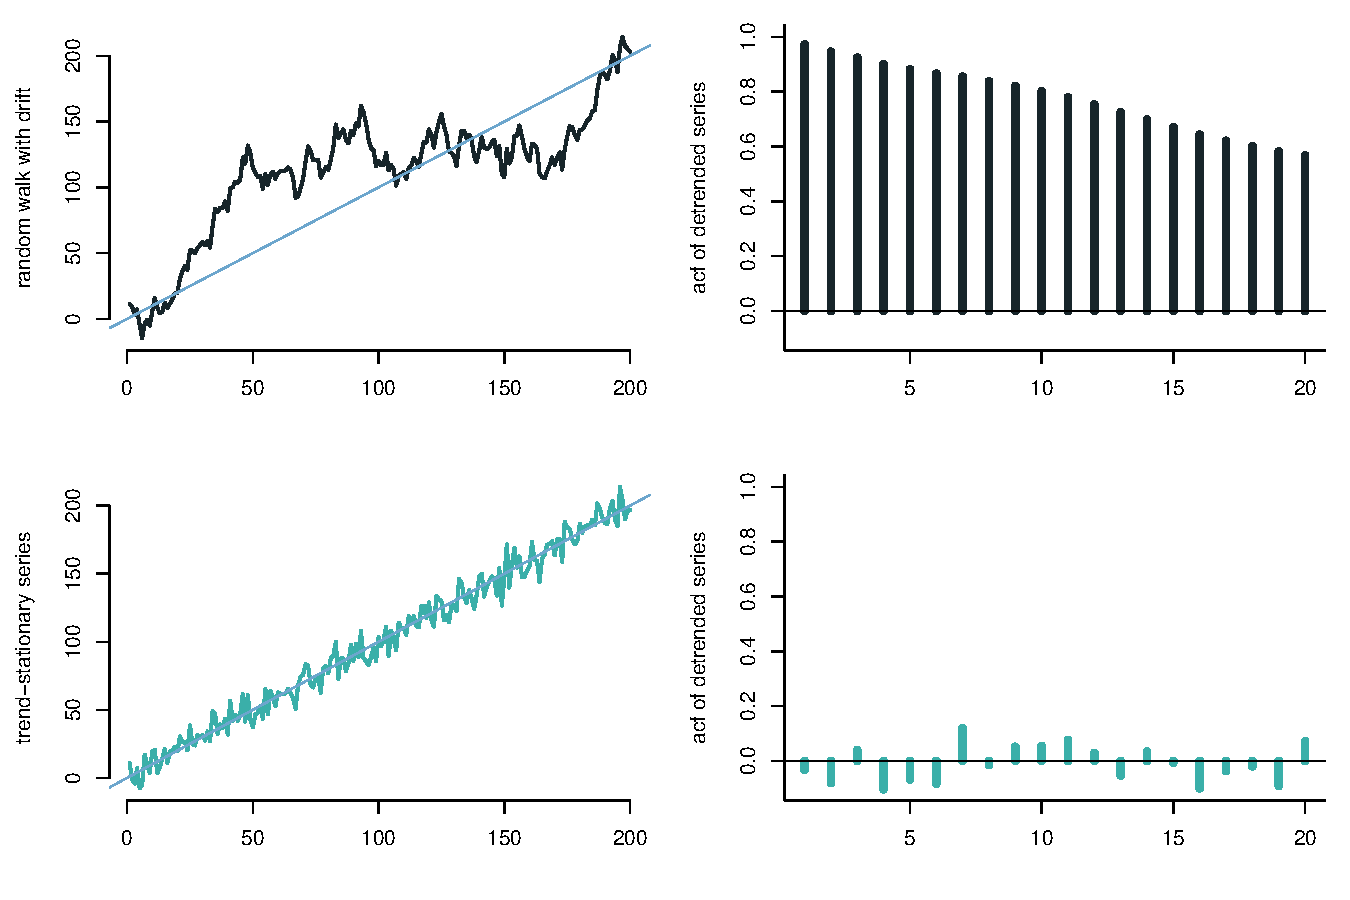
\includegraphics[scale=0.5, trim=0cm 0.6cm 0cm 0.5cm]{grphs/sim-tss-acfs.pdf}

{\color{mcxs2}Both series are generated using the same simulated shocks.}
\end{center}
\end{frame}
}





{\setbeamercolor{background canvas}{bg=mcxs5}
\begin{frame}

\begin{adjustwidth}{-0.5cm}{0cm}
%\FlushLeft
\vspace{8.3cm}\Large
\textbf{{\color{mcxs2}Inference} {\color{white}}}
\end{adjustwidth}

\end{frame}
}







\begin{frame}{Random walk process}

\textbf{Data generating process:} $y_t = y_{t-1} + \epsilon_t$

\bigskip\textbf{Estimated model.}
\begin{align*} 
y_t &= \alpha_1 y_{t-1} + \epsilon_t\\
\hat\alpha_1 &= \frac{\sum_{t=2}^{T}y_ty_{t-1}}{\sum_{t=2}^{T}y_{t-1}^2}
\end{align*} 

\textbf{Asymptotic distribution.}
$$ T\left(\hat\alpha_1 -1\right) \overset{d}{\rightarrow}\frac{B(1)^2-1}{2\int_{0}^{1}B(s)^2ds} $$

\begin{description}
\item[$T$]{\color{mcxs2}-- convergence rate implying} {\color{mcxs2}superconsistency}
\item[$B(s)$]{\color{mcxs2}-- Brownian motion}
\item[$B(1)^2-1 = \chi^2_1$]{\color{mcxs2}-- a $\chi^2$ distribution}
\item[$2\int_{0}^{1}B(s)^2ds$]{\color{mcxs2}-- non-normal distribution}
\end{description}

\end{frame}




\begin{frame}{Random walk process}

\textbf{Data generating process:} $y_t = y_{t-1} + \epsilon_t$

\bigskip\textbf{Estimated model.}
\begin{align*} 
y_t &= \alpha_1 y_{t-1} + \epsilon_t\\
\epsilon_t|y_{t-1}&\sim\mathcal{N}\left(0, \sigma_{\epsilon}^2\right)\\[1ex]
\hat\alpha_1 &= \frac{\sum_{t=2}^{T}y_ty_{t-1}}{\sum_{t=2}^{T}y_{t-1}^2}
\end{align*} 

\textbf{Likelihood function.}
$$ \alpha_1 \sim\mathcal{N}\left(\hat\alpha_1, \sigma_{\epsilon}^2(X'X)^{-1}\right) $$

\end{frame}







{\setbeamercolor{background canvas}{bg=mcxs5}
\begin{frame}

\begin{adjustwidth}{-0.5cm}{0cm}
%\FlushLeft
\vspace{8.3cm}\Large
\textbf{{\color{mcxs2}Illustration for} {\color{mcxs2}Australian real GDP}}
\end{adjustwidth}

\end{frame}
}





{\setbeamercolor{background canvas}{bg=mcxs5}
\begin{frame}{Australian real GDP}

\centering
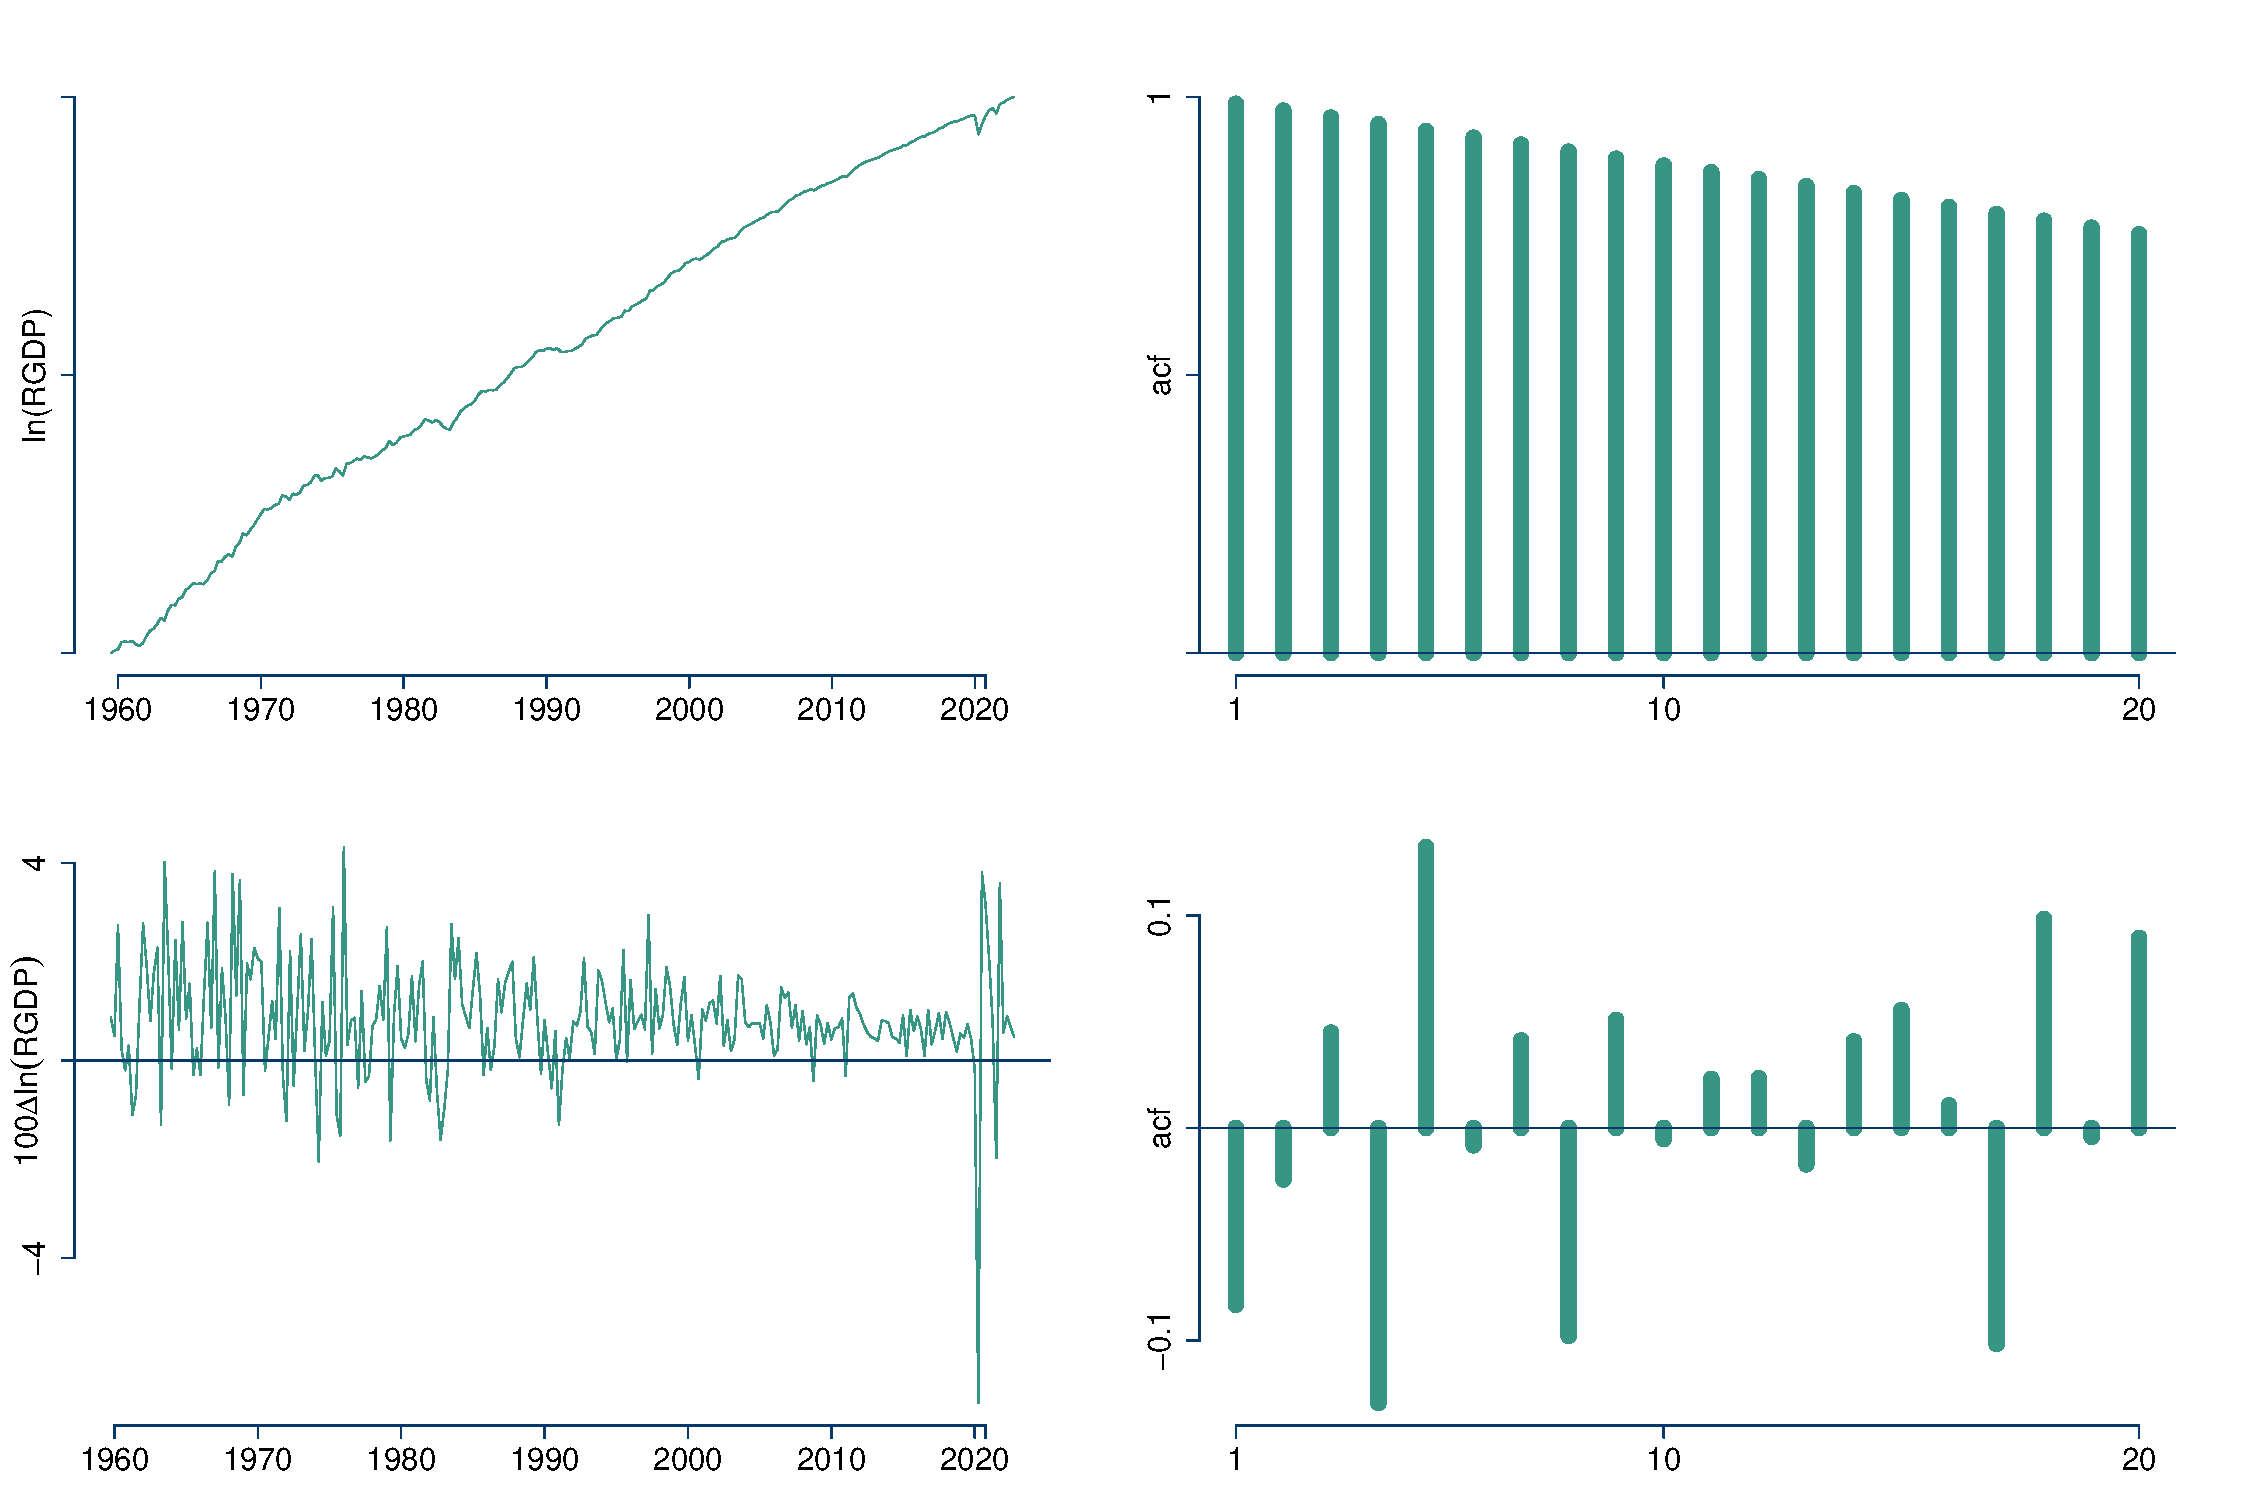
\includegraphics[scale=0.28]{grphs/05rgdp.pdf}

\bigskip\footnotesize{\color{mcxs2}Based on real GDP data for period Q3 1959 -- Q4 2022\\
Data source: Australian Macro Database \href{http://www.ausmacrodata.org/}{www.ausmacrodata.org}}
\end{frame}
}


{\setbeamercolor{background canvas}{bg=mcxs5}
\begin{frame}{Australian real GDP}

\centering
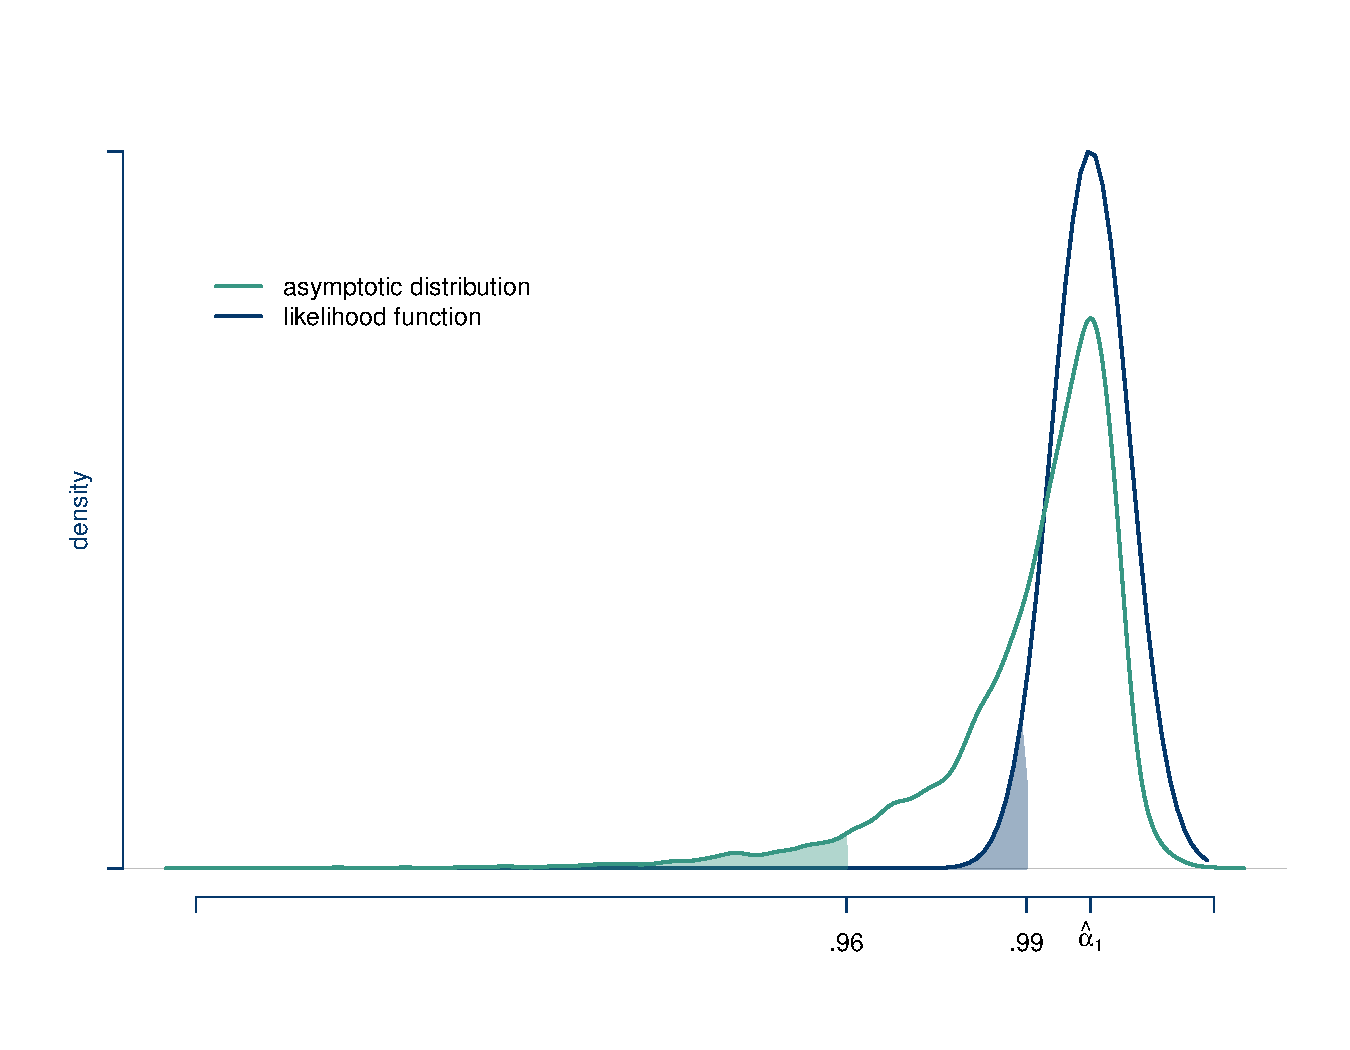
\includegraphics[scale=0.45]{grphs/05inference.pdf}

\end{frame}
}







{\setbeamercolor{background canvas}{bg=mcxs2}
\begin{frame}

\begin{adjustwidth}{-0.5cm}{0cm}
%\FlushLeft
\vspace{8.3cm}\Large
\textbf{{\color{mcxs1}A helicopter} {\color{mcxs3}tour}}
\end{adjustwidth}

\end{frame}
}







\begin{frame}{A helicopter tour: simulation setup}

\textbf{Data generating process.} \small
\begin{align*}
y_t &= \rho y_{t-1} + \epsilon_t \quad\text{\color{mcxs2}and}\quad \epsilon_t\sim\mathcal{N}\left(0, \sigma^2_{\epsilon}=1\right)\\
\rho &\in\{ .8, .81, .82, \dots, 1.09, 1.1 \}\quad\text{\color{mcxs2}-- a grid of 31 values for $\rho$}\\
y_0 &= 0
\end{align*}

\smallskip\normalsize\textbf{Matrix notation.}\small
\begin{align*}
\mathbf{R} y &=  E \quad\text{\color{mcxs2}and}\quad E\sim\mathcal{N}\left(\mathbf{0}_T, I_T\right)\\
y &=  \mathbf{R} ^{-1}E \quad\text{\color{mcxs2}-- generate data from AR(1)}  {\color{mcxs3}DGP}\\[1ex]
\underset{\color{mcxs2}(T\times T)}{\mathbf{R}} &= \begin{bmatrix} 1&0& 0 &\dots&0&0 \\ -\rho &1&0&\dots&0&0\\ 0&-\rho &1&\dots&0&0 \\ \vdots&\vdots&\vdots&\ddots&\vdots&\vdots\\ 0&0&0&\dots &-\rho&1\end{bmatrix}
\qquad y= \begin{bmatrix}y_1\\y_2\\ \vdots \\ y_{T-1}\\y_T \end{bmatrix}
\end{align*}

\end{frame}





\begin{frame}{A helicopter tour: simulation setup}

\textbf{Estimated parameter.} \small
 \begin{align*}
\hat\rho_{ML} &= (X'X)^{-1}X'Y\\
Y' &= \begin{bmatrix} y_2 & y_3 & \dots& y_T \end{bmatrix}\\
X' &= \begin{bmatrix} y_1 & y_2 & \dots& y_{T-1} \end{bmatrix}
\end{align*}

\smallskip\normalsize\textbf{Generate the graph.}\small
\begin{description}
\item[Generate] $S=50,000$ {\color{mcxs2}times} $T=100$ {\color{mcxs2}random numbers from} $\mathcal{N}(0,1)$
\item[Create] {\color{mcxs2}For} $50,000$ $T\times1$ {\color{mcxs2}normal vectors and for 31 values of} $\rho$ {\color{mcxs2}from the grid compute} $y$ {\color{mcxs2}according to the} {\color{mcxs3}DGP}
\item[Estimate] $\hat\rho_{ML}$ {\color{mcxs2}for each of the generated} $y$ {\color{mcxs2}vector} 
\item[Compute histograms] {\color{mcxs2}of} $\hat\rho_{ML}$ {\color{mcxs2}for each of grid values} $\rho$ {\color{mcxs2}using bins:}
$ (-\infty,.795], (.795, .805], (.805, .815], \dots , (1.095, 1.105], , (1.105, \infty] $
\item[Plot] {\color{mcxs2}the joint distribution of} $\hat\rho_{ML}$ {\color{mcxs2}and} $\rho$
\end{description}

\end{frame}


{\setbeamercolor{background canvas}{bg=mcxs4}
\begin{frame}{A helicopter tour}
\centering
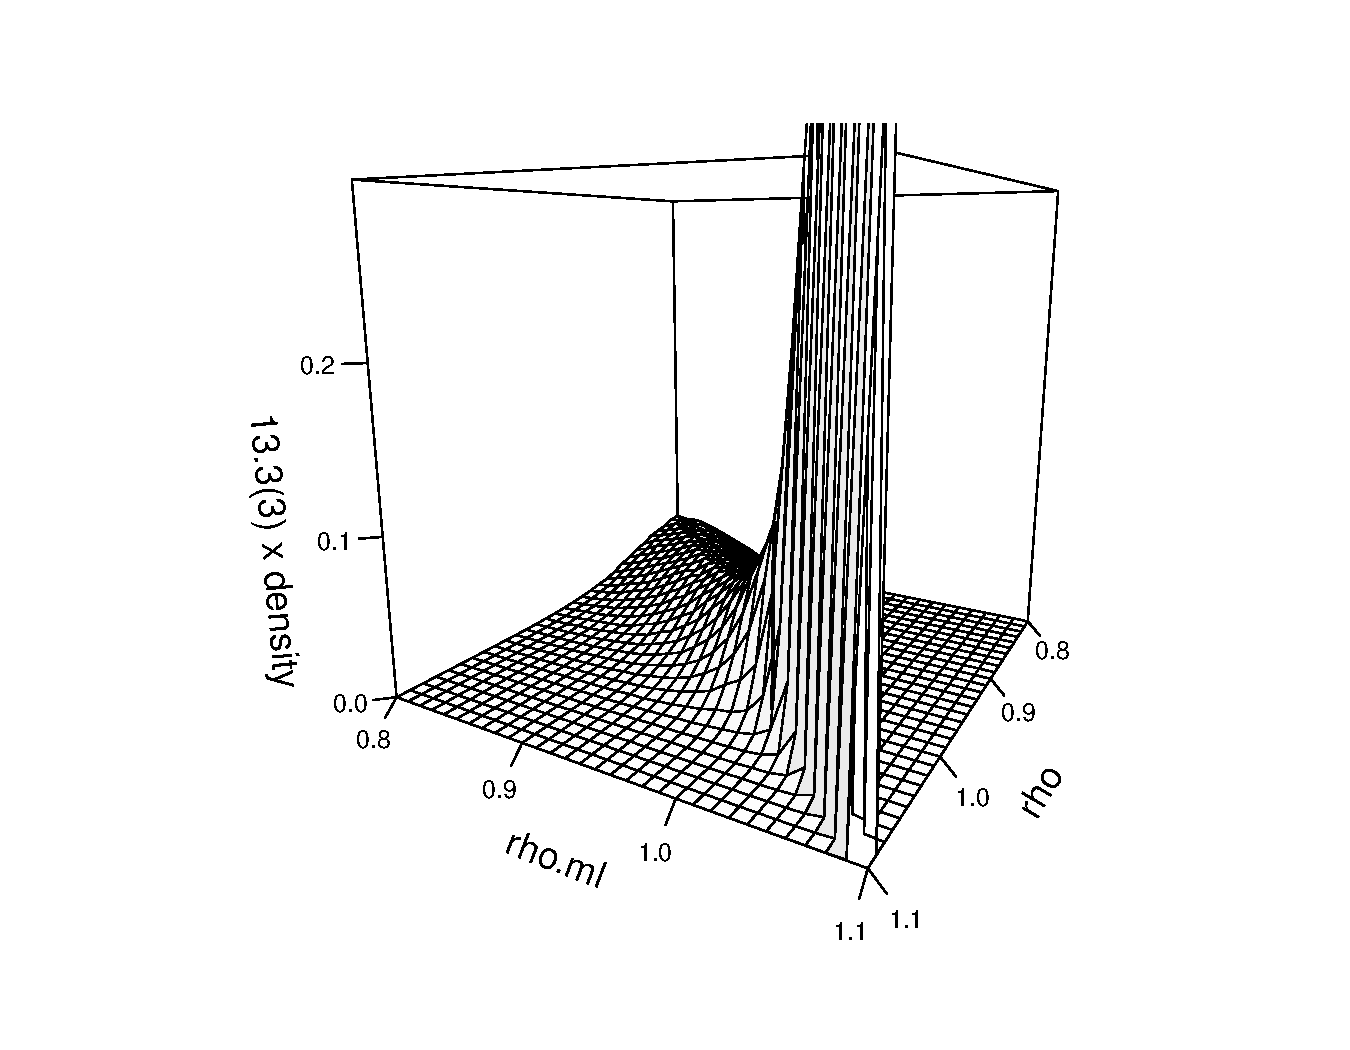
\includegraphics[scale=0.45]{grphs/05behind-nopdf}

\end{frame}
}





\begin{frame}{A helicopter tour: conditional distributions}

$${\color{mcxs2}p(\hat\rho_{ML}|\rho=1)}$$\small
\begin{description}
\item[Is a simulated] {\color{mcxs2}distribution of MLE of} $\rho$ {\color{mcxs2}given that the data is generated using a fixed value of} $\rho=1$
\item[Is equivalent] {\color{mcxs2}to the asymptotic distribution of} $\hat\rho_{ML}$ {\color{mcxs2}with} $T\rightarrow\infty$
\item[Is used] {\color{mcxs2}to compute the critical values for unit root tests}
\end{description}


\normalsize$${\color{mcxs1}p(\rho|\hat\rho_{ML}=1)}$$\small
\begin{description}
\item[Is equivalent] to the posterior distribution of $\rho$ given that data $y$ is such that $\hat\rho_{ML}=1$ and $\sigma^2_{\epsilon}$ is fixed to 1
\item[Prior distribution] in this case is set to an improper distribution $p(\rho)\propto1$, e.g., $p(\rho)=1$
\item[Posterior distribution] is then proportional to $\exp\left\{ -\frac{1}{2}\left(\rho-\hat\rho_{ML}\right)'X'X\left(\rho-\hat\rho_{ML}\right) \right\}$
\end{description}

\end{frame}




{\setbeamercolor{background canvas}{bg=mcxs4}
\begin{frame}{A helicopter tour: joint distribution}
\centering
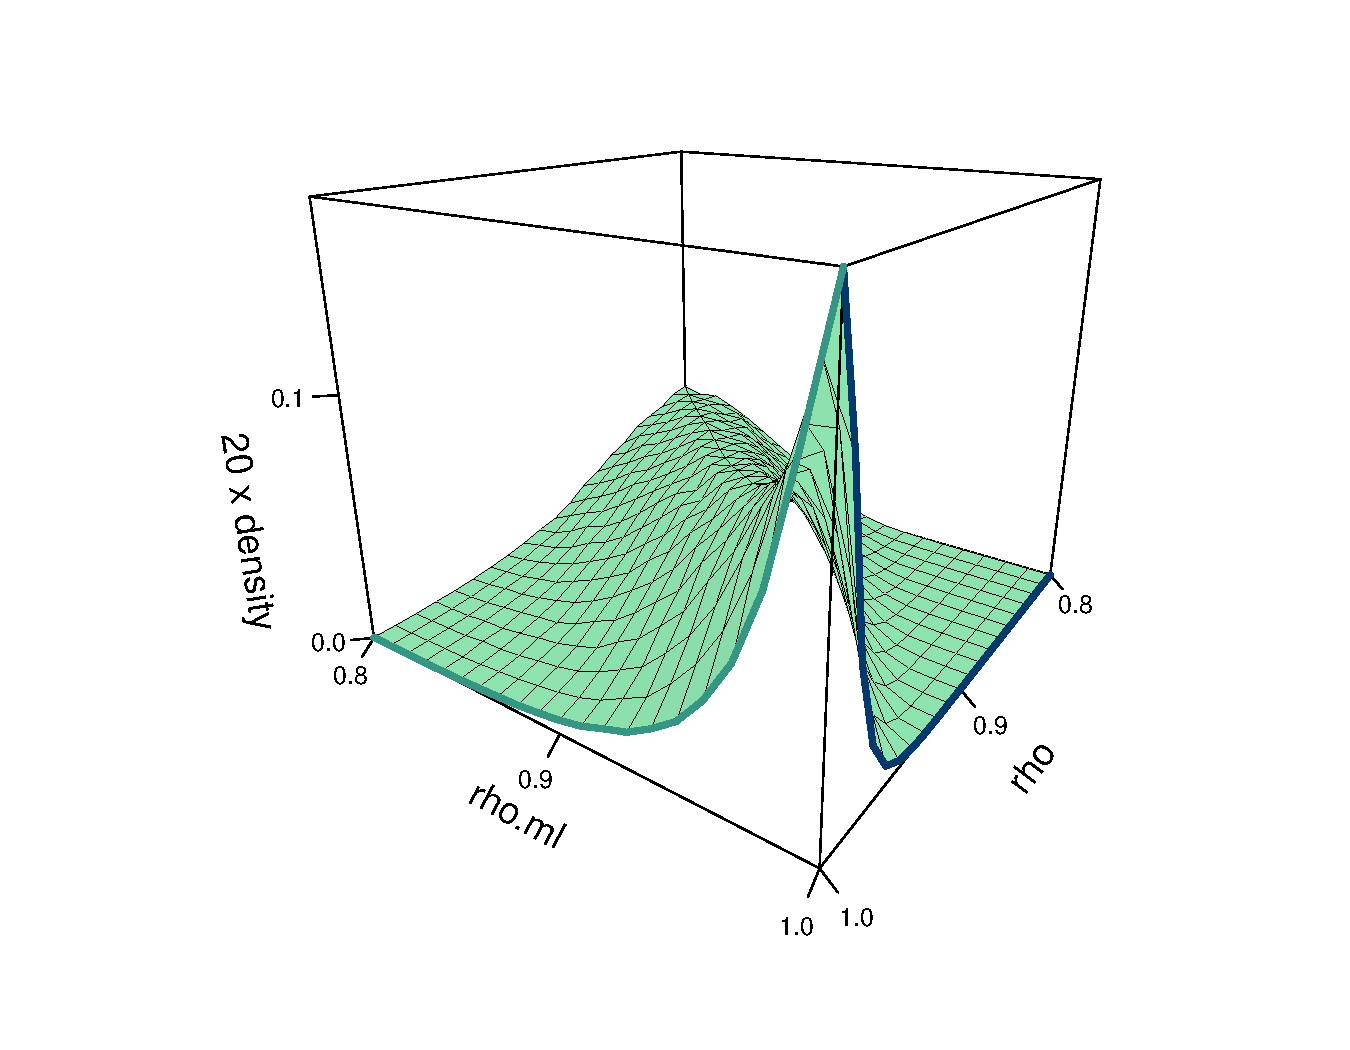
\includegraphics[scale=0.45]{grphs/05f1}

$ {\color{mcxs2}p(\hat\rho_{ML}|\rho=1)} \qquad {\color{mcxs1}p(\rho|\hat\rho_{ML}=1)} $
\end{frame}
}





{\setbeamercolor{background canvas}{bg=mcxs4}
\begin{frame}{A helicopter tour: asymmetry}
\centering
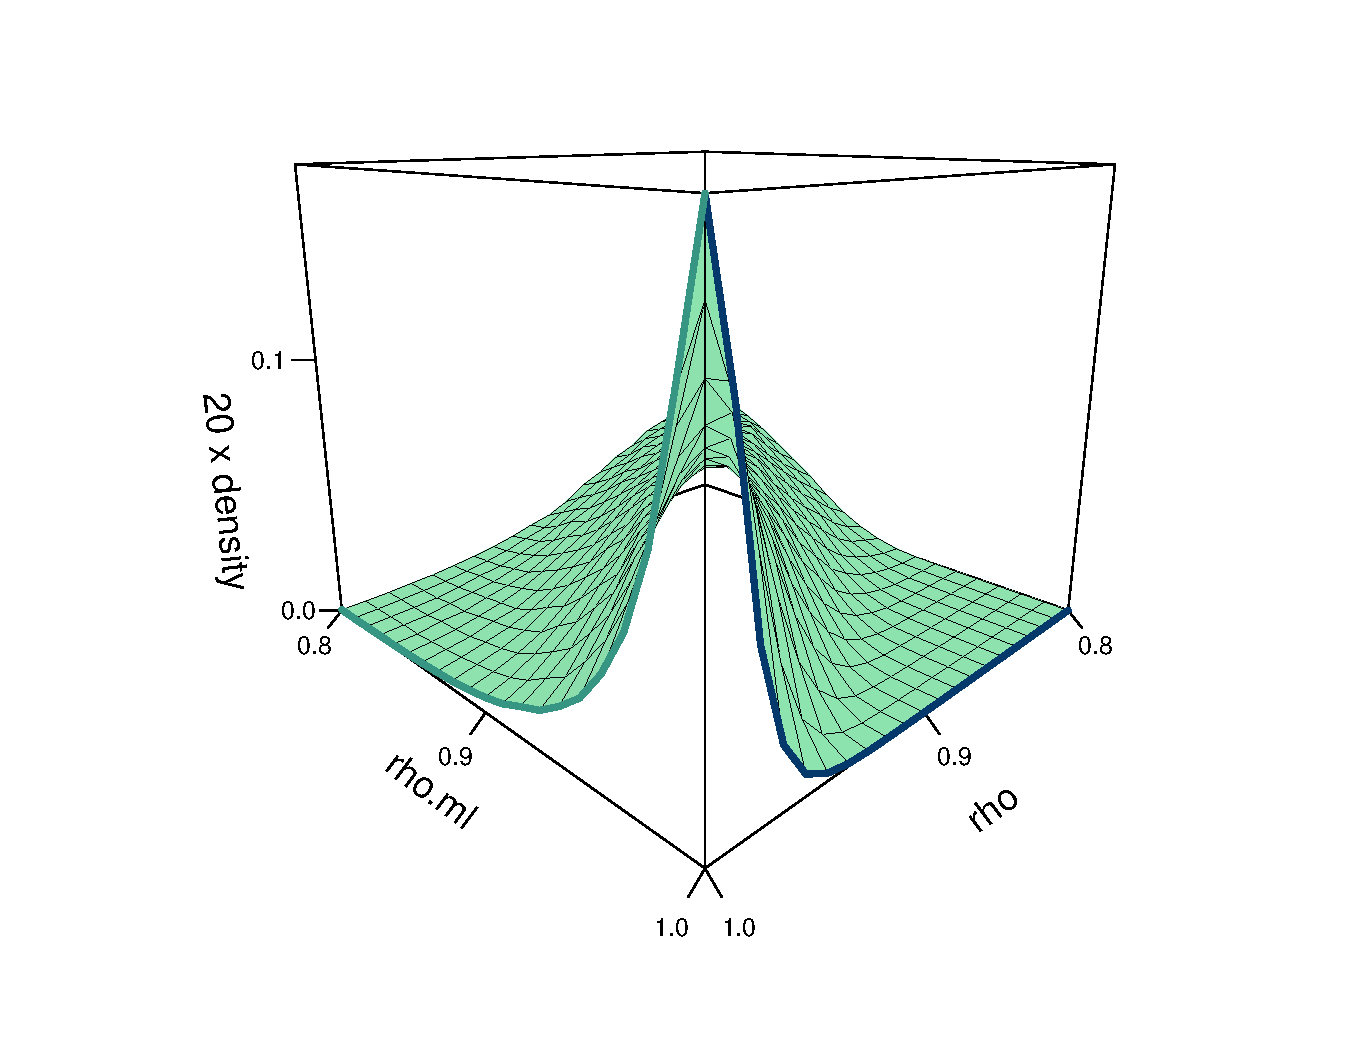
\includegraphics[scale=0.45]{grphs/05f2}

$ {\color{mcxs2}p(\hat\rho_{ML}|\rho=1)} \qquad {\color{mcxs1}p(\rho|\hat\rho_{ML}=1)} $
\end{frame}
}

{\setbeamercolor{background canvas}{bg=mcxs4}
\begin{frame}{A helicopter tour: asymptotic distribution}
\centering
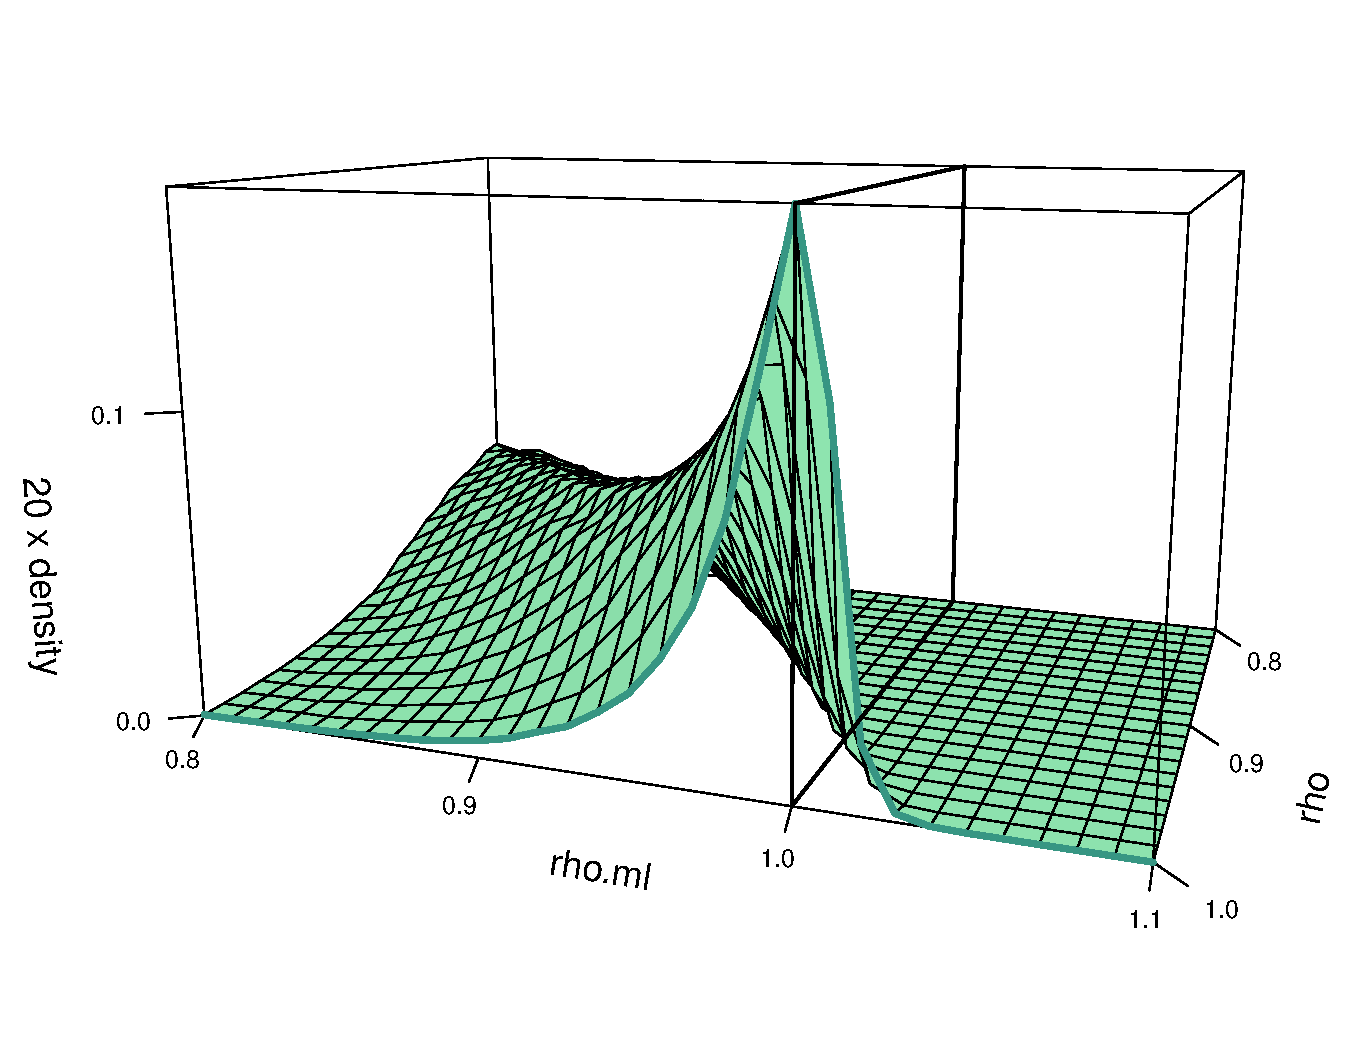
\includegraphics[scale=0.45]{grphs/05f3}

$ {\color{mcxs2}p(\hat\rho_{ML}|\rho=1)} $
\end{frame}
}



{\setbeamercolor{background canvas}{bg=mcxs4}
\begin{frame}{A helicopter tour: posterior distribution}
\centering
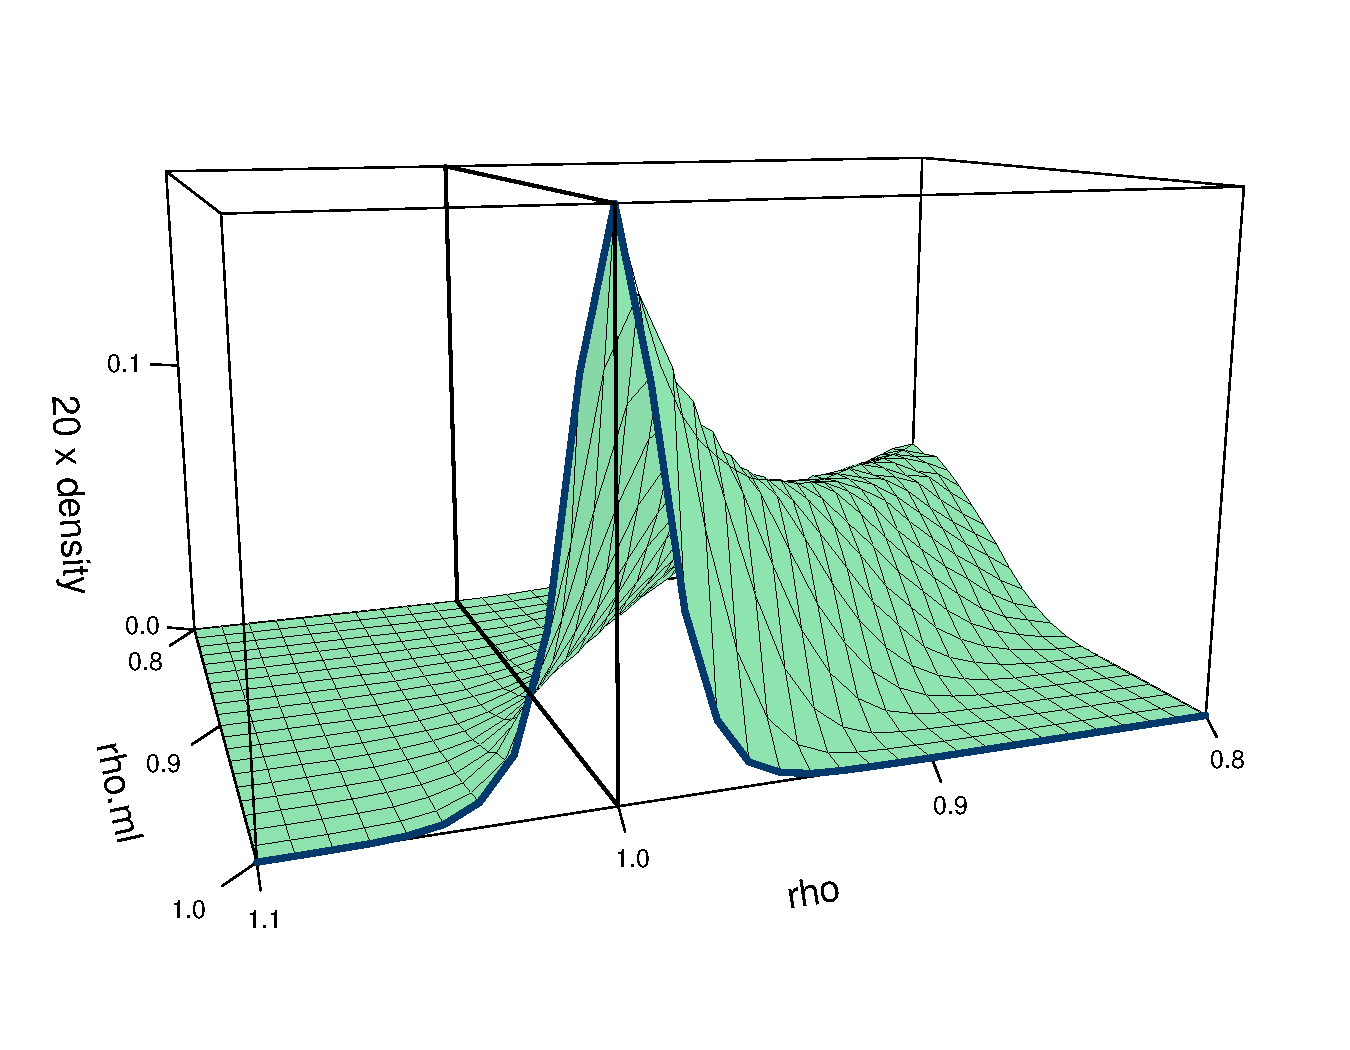
\includegraphics[scale=0.45]{grphs/05f4}

$  {\color{mcxs1}p(\rho|\hat\rho_{ML}=1)} $
\end{frame}
}


{\setbeamercolor{background canvas}{bg=mcxs4}
\begin{frame}{A helicopter tour: posterior distribution}
\centering
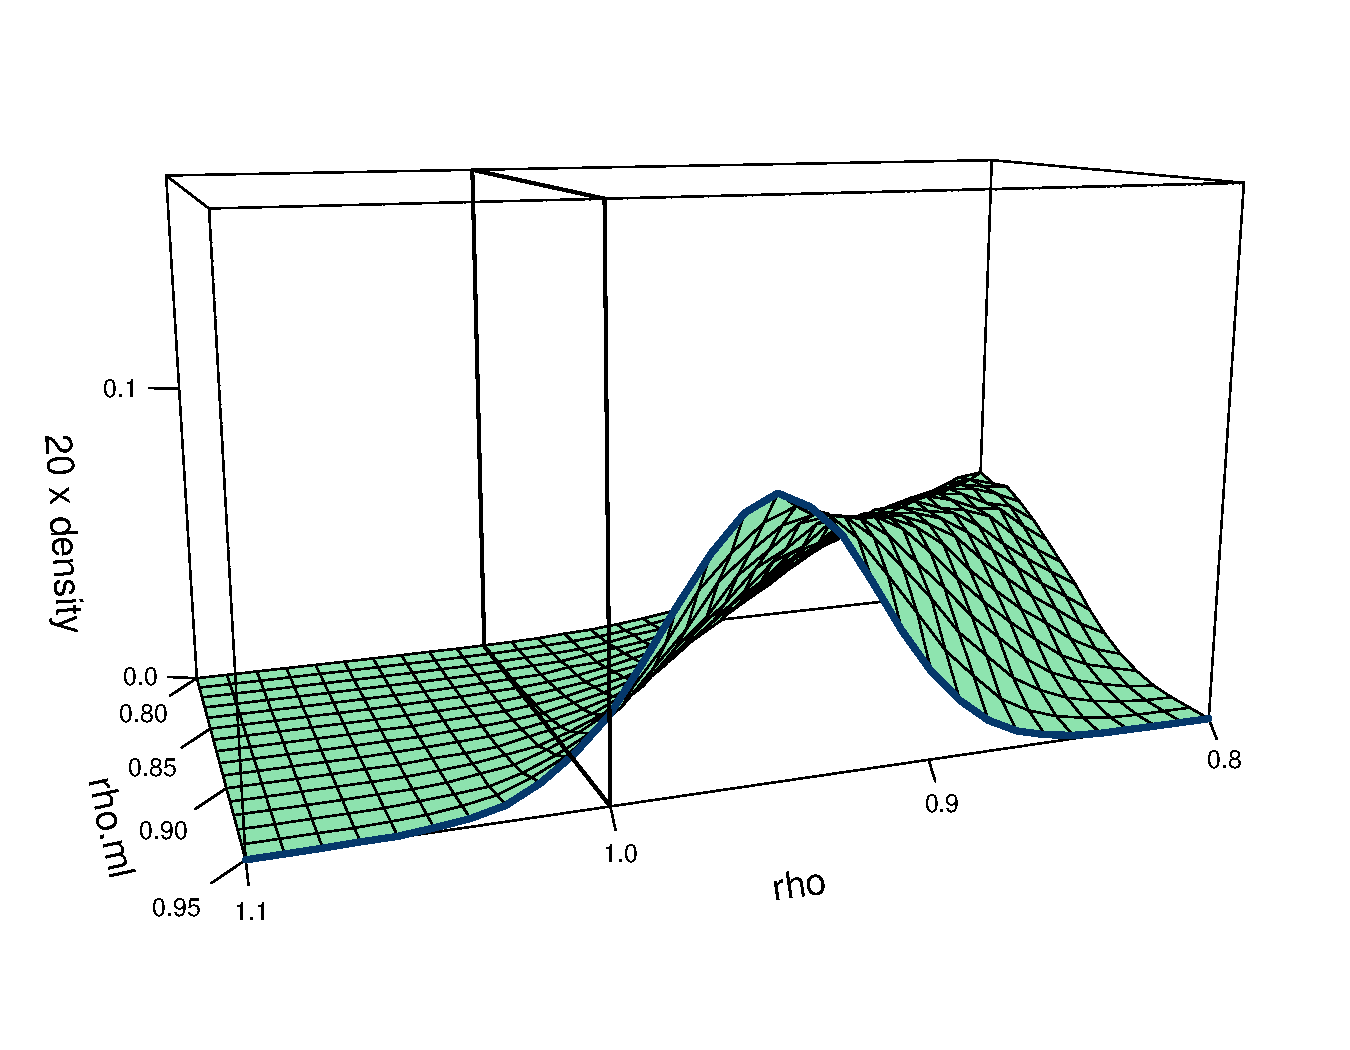
\includegraphics[scale=0.45]{grphs/05f5}

$  {\color{mcxs1}p(\rho|\hat\rho_{ML}=.95)} $
\end{frame}
}

{\setbeamercolor{background canvas}{bg=mcxs4}
\begin{frame}{A helicopter tour}
\centering
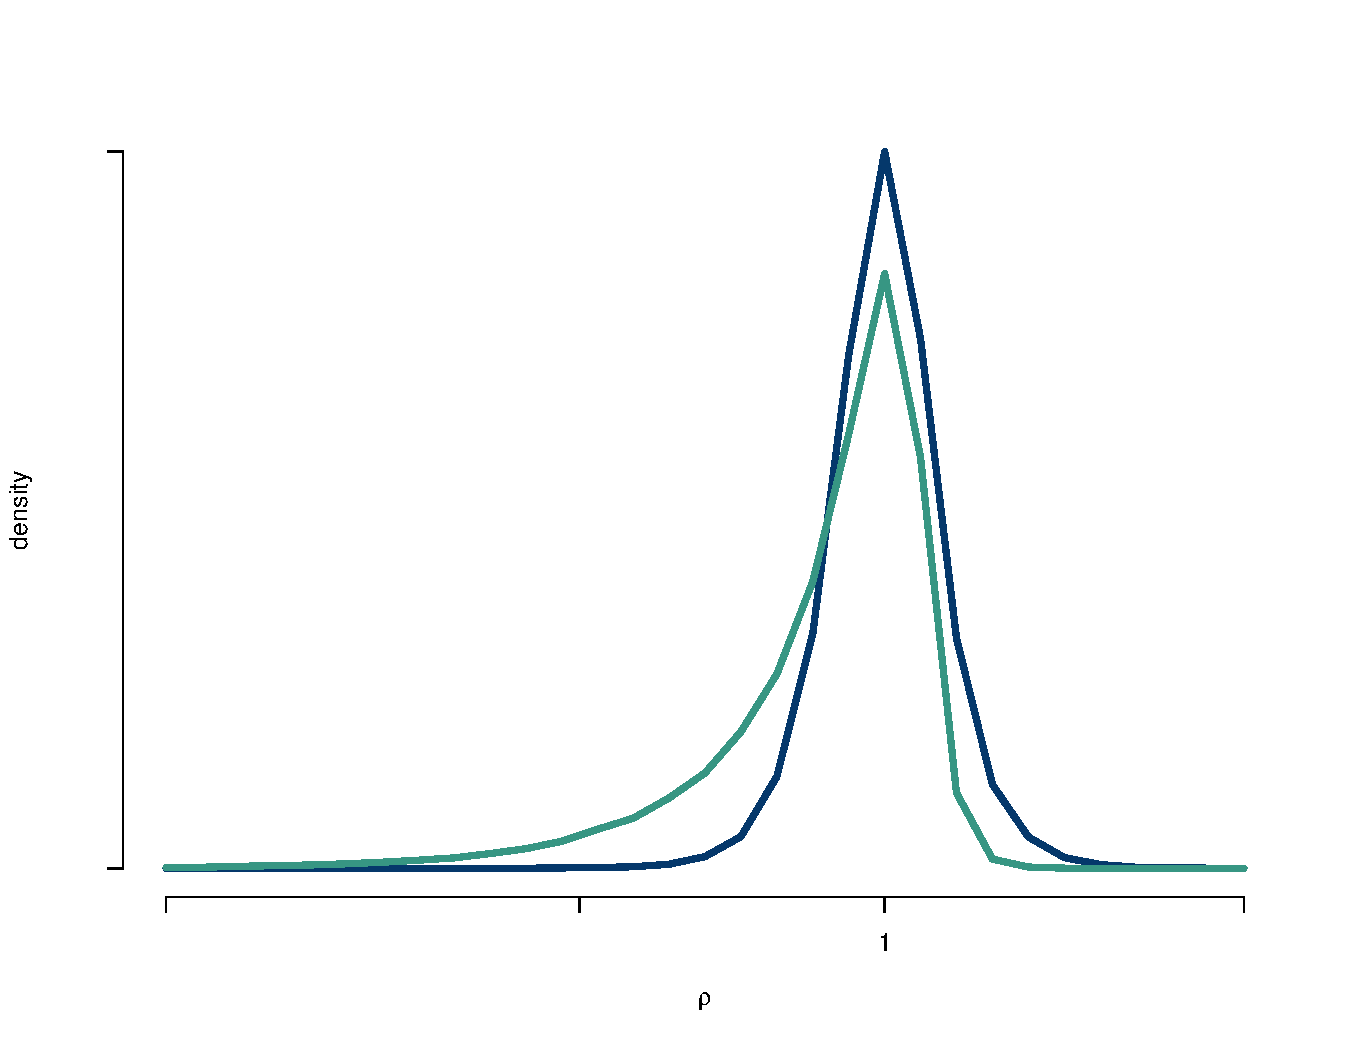
\includegraphics[scale=0.45]{grphs/05f6}

$ {\color{mcxs2}p(\hat\rho_{ML}|\rho=1)} \qquad {\color{mcxs1}p(\rho|\hat\rho_{ML}=1)} $
\end{frame}
}


{\setbeamercolor{background canvas}{bg=mcxs4}
\begin{frame}{A helicopter tour}
\centering
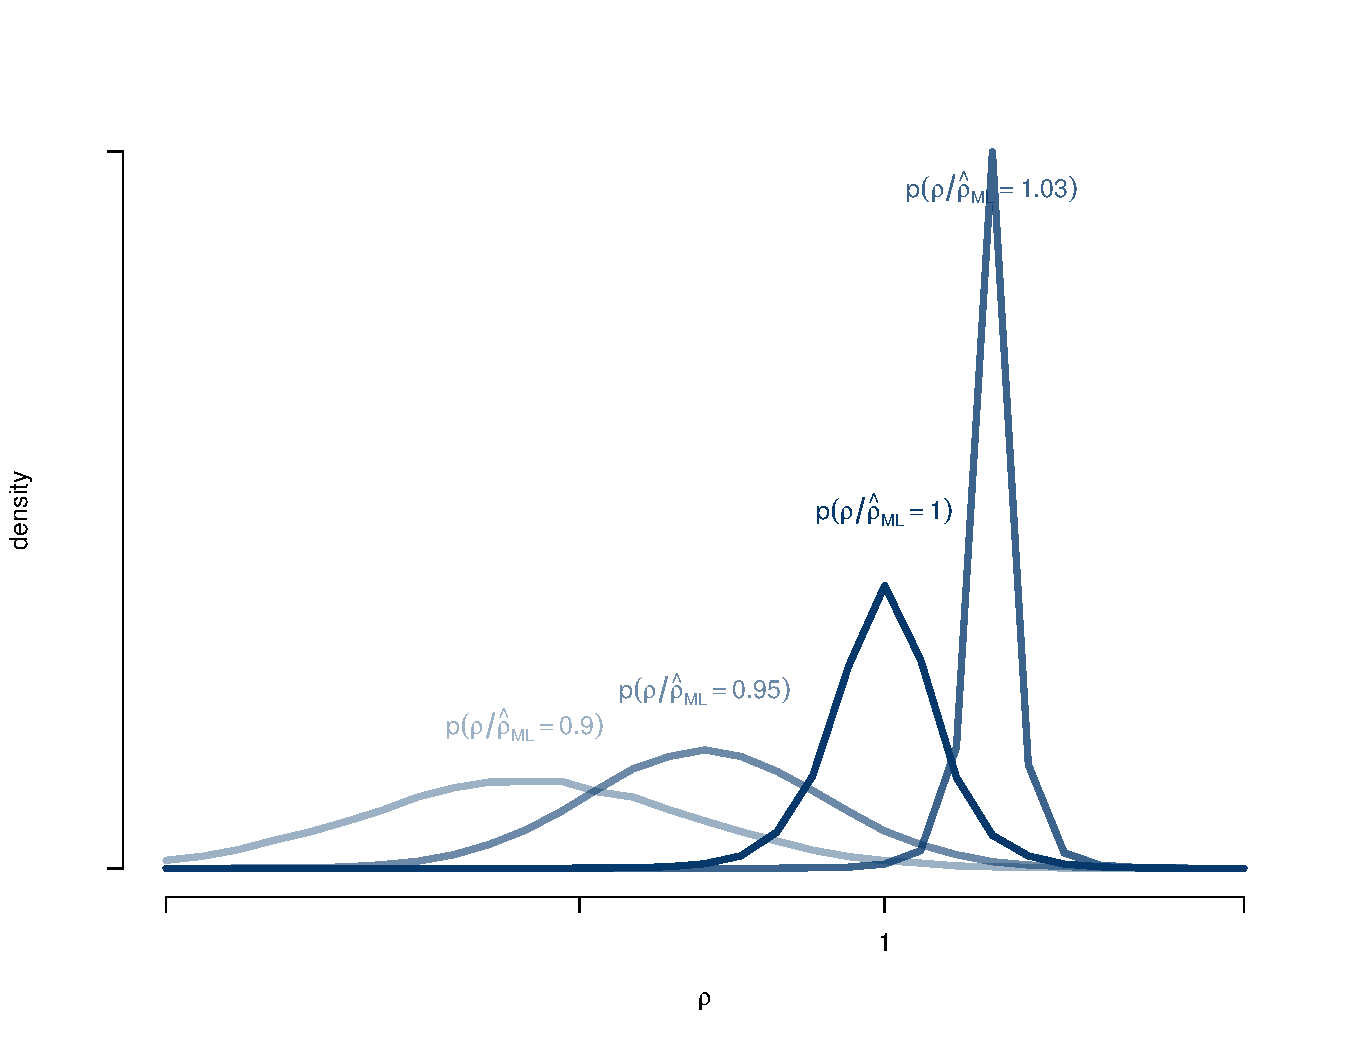
\includegraphics[scale=0.45]{grphs/05f7}

%$ {\color{mcxs2}p(\hat\rho_{ML}|\rho=1)} \qquad {\color{Blue}p(\rho|\hat\rho_{ML}=.95)} $
\end{frame}
}


{\setbeamercolor{background canvas}{bg=mcxs4}
\begin{frame}{A helicopter tour: behind the scenes}
\centering
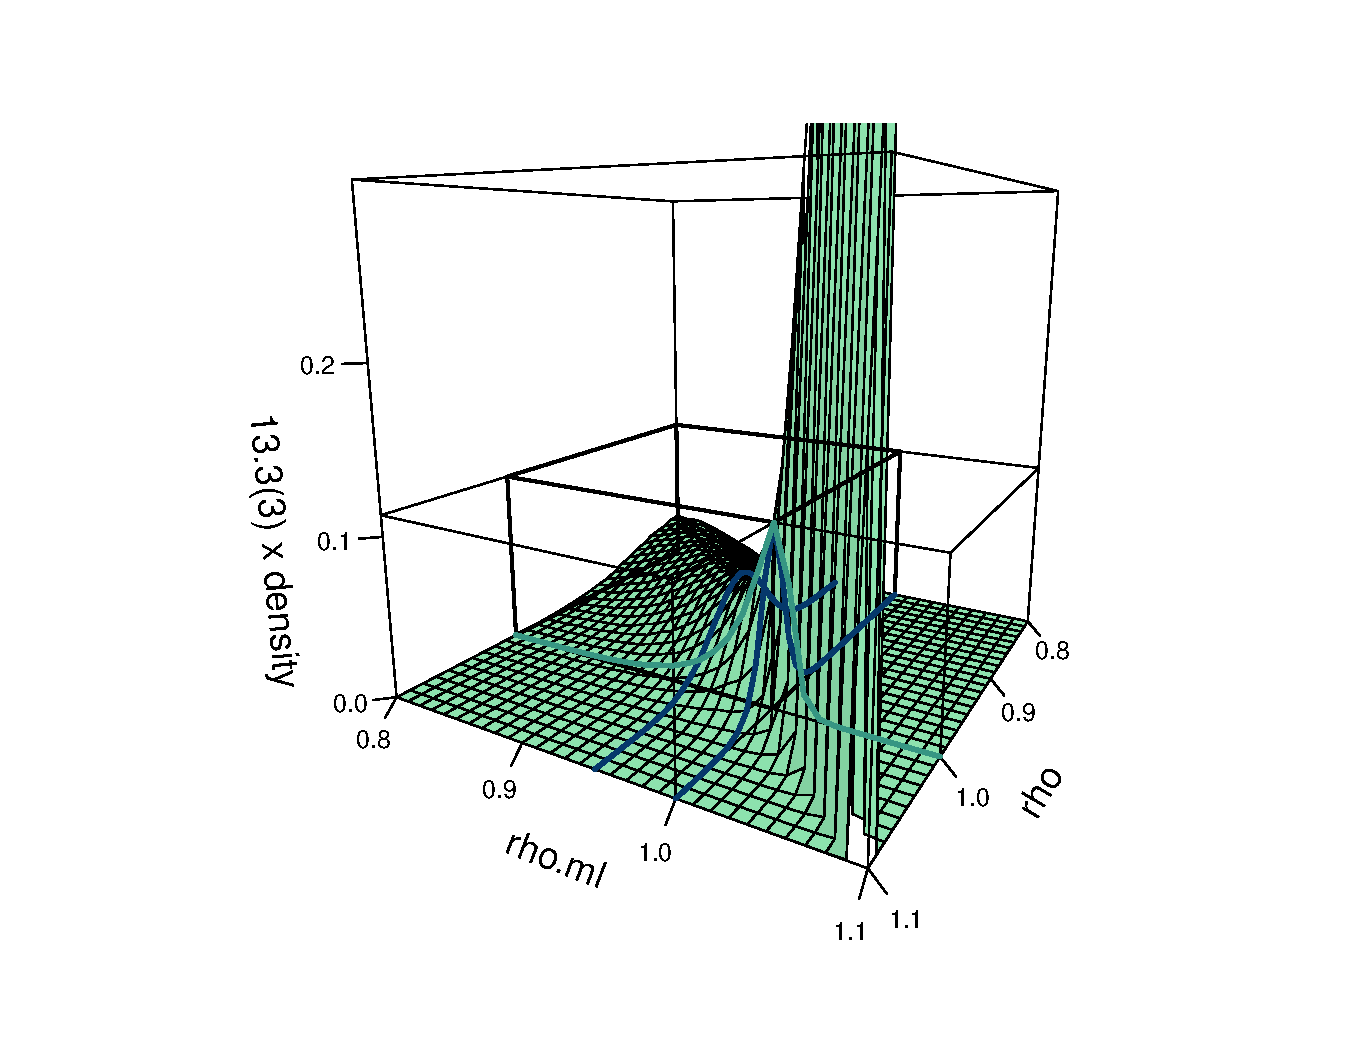
\includegraphics[scale=0.45]{grphs/05behind}

$ {\color{mcxs2}p(\hat\rho_{ML}|\rho=1)} \qquad {\color{mcxs1}p(\rho|\hat\rho_{ML}=1)} \qquad {\color{mcxs1}p(\rho|\hat\rho_{ML}=.95)} $
\end{frame}
}

























{\setbeamercolor{background canvas}{bg=mcxs5}
\begin{frame}{Random walk process}

\begin{description}
\item[Autoregressions] {\color{mcxs2}provide convenient parameterization for modeling decaying patterns in autocorrelations of time series}

\bigskip\item[Random walk process] {\color{mcxs2}imply long-memory and unit autocorrelations at all lags}

\bigskip\item[Note: seemingly conflicting evidence] {\color{mcxs2} from the asymptotic distribution and the likelihood function}

\smallskip\item[The posterior] {\color{mcxs2}distribution is normal}

\smallskip\item[Unit-root inference] {\color{mcxs2}seems to be the only case when Bayesian and frequentist approaches do not converge asymptotically}

\end{description}
\end{frame}
}



\end{document} 